\begin{inhalt}
\renewcommand*\chapterpagestyle{scrheadings}
\chapter{Website}


\section{Signup}

Für Das Zuordnen der jeweiligen Benutzer ist es Notwendig das die User Sich einloggen können. Dafür muss ein Anmelde Komponente erstellt werden.

\begin{figure}[!htb]
\centering
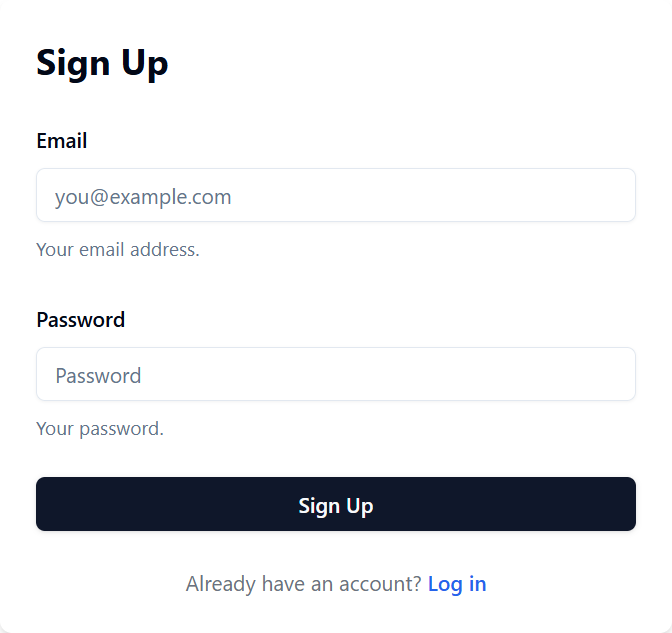
\includegraphics[width=1\textwidth]{files/Thomas/pics/Website/Signup/sign-up.png}
\caption[Bildbezeichnung für Abbildungsverzeichnis]{}
\label{fig:gehaeuse_internet_bild}
\end{figure}

Zur Validierung der Eingaben in den Feldern für \texttt{E-Mail} und \texttt{Passwort} wird die Bibliothek \textbf{Zod} verwendet. Dabei überprüft \textbf{Zod}, ob das E-Mail-Feld eine syntaktisch gültige E-Mail-Adresse enthält und ob das Passwortfeld einen String mit einer Mindestlänge von sechs Zeichen beinhaltet.


\begin{lstlisting}[style=mytsx]
const formSchema = z.object({
  email: z.string().email({
    message: "Please enter a valid email.",
  }),
  password: z.string().min(6, {
    message: "Password must be at least 6 characters.",
  }),
})
\end{lstlisting}
\index{Code Snippet 1@\hyperref[code:snippet1]{Snippet 1}}

Für den Registrierungsvorgang wurde eine Funktion implementiert, die die eingegebene E-Mail-Adresse sowie das Passwort entgegennimmt und diese über eine Funktion des Supabase-Auth-Services im System registriert.


\begin{lstlisting}[style=mytsx]
export async function insert_user(email: string, password: string) {
  const supabase = await createClient();
  const { error } = await supabase.auth.signUp({
    email,
    password,
  });
  return error;
}
\end{lstlisting}

Nachdem der Nutzer erfolgreich registriert wurde, erfolgt eine Weiterleitung auf die Seite \texttt{/checkyouremails}, um ihn darüber zu informieren, dass er seine E-Mails überprüfen soll.

\begin{lstlisting}[style=mytsx]
      router.push("checkyouremails");
\end{lstlisting}

\subsection{Check Your Emails}

Auf dieser Seite checkt die Seite ob im Table profiles \ref{}


\section{Login}
Für Das Zuordnen der jeweiligen Benutzer ist es Notwendig das die User Sich einlogen können

\begin{figure}[!htb]
\centering
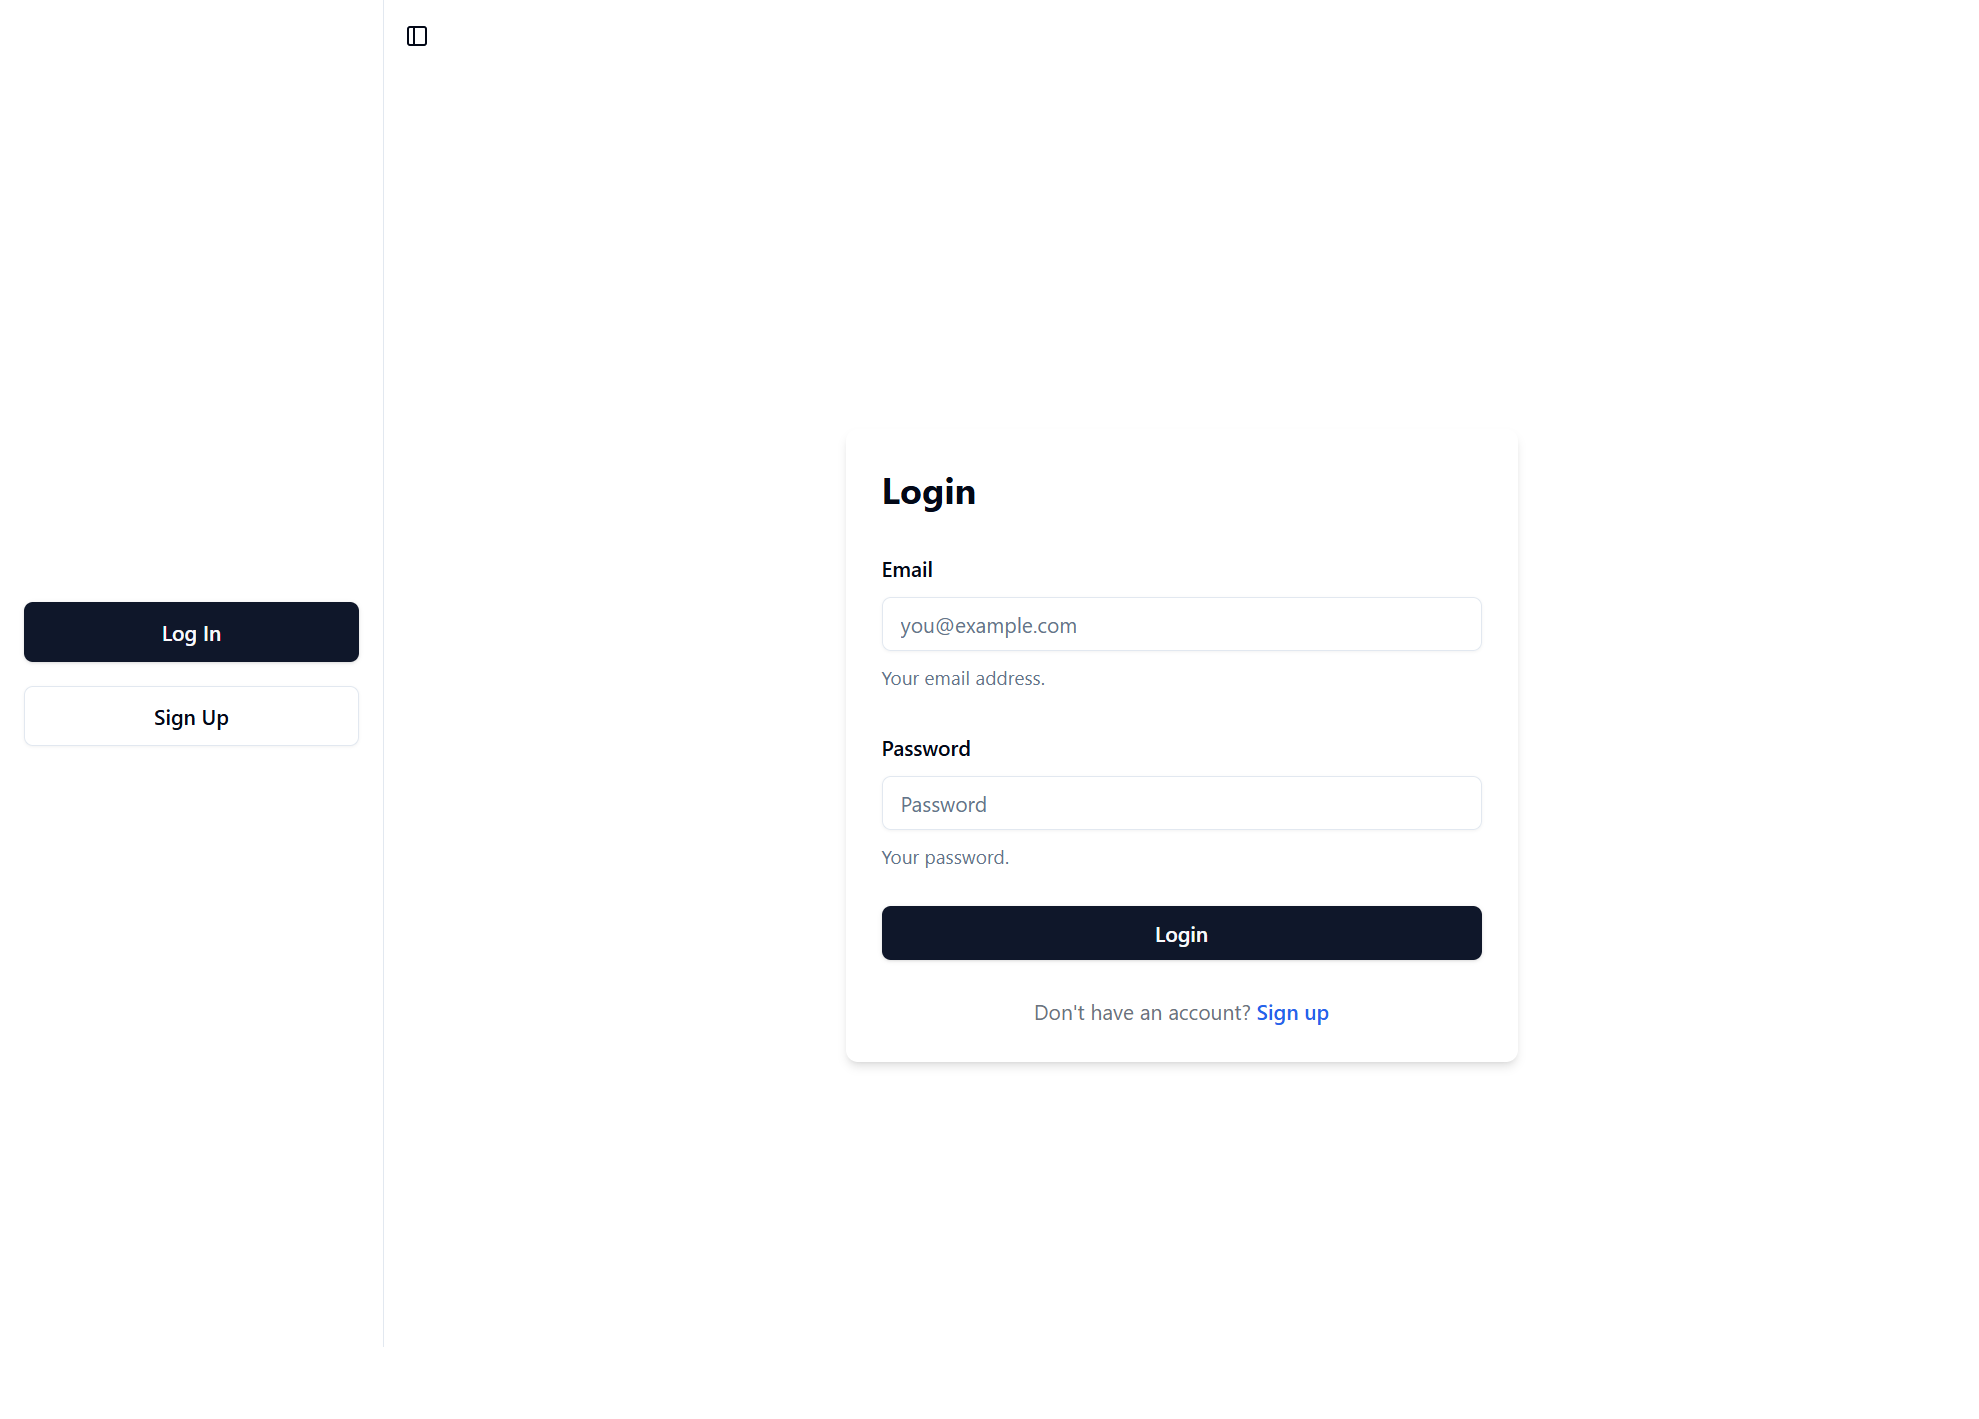
\includegraphics[width=1\textwidth]{files/Thomas/pics/Website/Login/login-screen.png}
\caption[Bildbezeichnung für Abbildungsverzeichnis]{}
\label{fig:gehaeuse_internet_bild}
\end{figure}

Dafür wurde ein Login Komponente erstellt.

\begin{figure}[!htb]
\centering
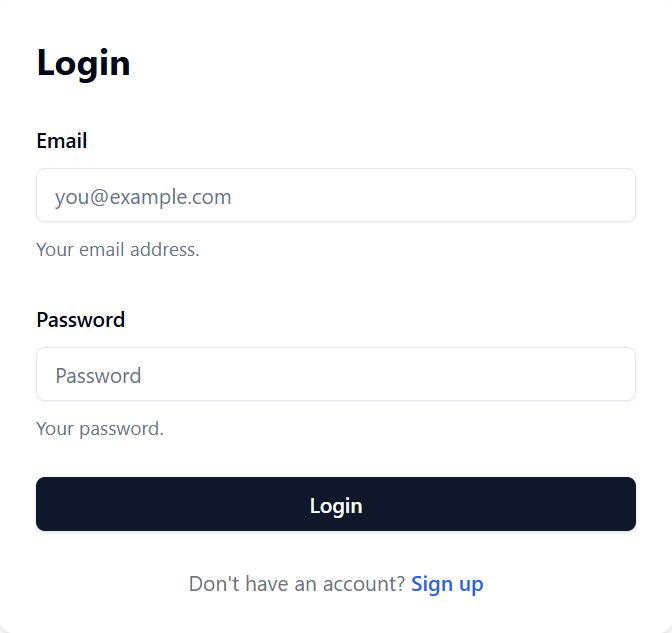
\includegraphics[width=1\textwidth]{files/Thomas/pics/Website/Login/login.png}
\caption[Bildbezeichnung für Abbildungsverzeichnis]{}
\label{fig:gehaeuse_internet_bild}
\end{figure}

Für das Login Komponent wurde Zod für die überprüfung von 

\begin{lstlisting}[style=mytsx]
export async function login_user(email: string, password: string) {
  const supabase = await createClient();
  const { error } = await supabase.auth.signInWithPassword({
    email,
    password,
  });
  return error;
}
\end{lstlisting}






























\section{Admin Dashboard}

Das Admin Dashboard ist dafür da um alle User, Geräte, Klassen, Abteilungen und Schulen zu Erstellen oder zu Löschen. 

\subsection{Tables}

\subsubsection{School}

\subsubsection{Departments}

\subsubsection{Class}

\subsubsection{Devices}

\subsubsection{User}

\subsection{Create}

Auf allen Seiten der Administrationsoberfläche kommt ein spezielles \emph{Create}-Component zum Einsatz, das jeweils für die Erstellung einzelner Objekte zuständig ist. Die Namensgebung folgt dabei einer klaren Konvention, beispielsweise \texttt{create-school.tsx} für den Schulbereich. Der Begriff \emph{Create} leitet sich aus dem englischen Begriff „erstellen“ ab, was die primäre Funktion dieser Komponente treffend beschreibt.

Jede dieser Komponenten ist individuell auf die jeweilige Entität zugeschnitten, um eine optimale Handhabung und Validierung der Eingabedaten zu gewährleisten. Nach erfolgreicher Erstellung werden die eingegebenen Daten in der Supabase-Datenbank gespeichert, was eine konsistente und strukturierte Datenhaltung ermöglicht.

\subsubsection{School}






Im Folgenden wird erläutert, wie in diesem Projekt die Autovervollständigung für Adressen mithilfe der Google API implementiert wurde.

\subsubsection{Google API für Autovervollständigung}

Für die Implementierung der Autovervollständigung wurde das npm-Package \texttt{react-google-maps-api} eingesetzt. Diese Lösung bietet eine einfache Möglichkeit, Google-basierte Adressvorschläge in das Projekt zu integrieren. Hierfür musste im Google-Dashboard die neue Places API aktiviert werden, da seit dem 17.03.2025 keine Legacy-Version mehr verfügbar ist.

Das verwendete \texttt{AddressAutocomplete}-Component stellt ein Beispiel für die Umsetzung dar:

\begin{lstlisting}[style=mytsx]
<AddressAutocomplete
  value={field.value}
  onChange={field.onChange}
  onBlur={field.onBlur}
/>
\end{lstlisting}

Mit diesem Component kann der Benutzer eine Adresse oder einen Ort suchen. Google liefert daraufhin entsprechende Vorschläge, die anschließend in einem JSON-Format gespeichert werden. Ein exemplarischer Aufbau des JSON-Objekts sieht folgendermaßen aus:

\begin{lstlisting}[style=myjson]
{
  location: {
    address: "",
    location: {
      latitude: 0,
      longitude: 0,
    },
    address_id: null,
  },
}
\end{lstlisting}

Die Validierung und Verwaltung der erhaltenen Daten erfolgt mittels \texttt{Zod} (siehe Abschnitt \ref{subsec:Zod}). Dies gewährleistet, dass die eingegebene Adresse den Mindestanforderungen entspricht und die Geodaten korrekt formatiert sind. Im folgenden Listing wird die Validierung mittels \texttt{Zod} veranschaulicht:

\begin{lstlisting}[style=myjson]
{
  location: z.object({
    address: z.string().min(2, {
      message: "Please enter a valid address.",
    }),
    location: z.object({
      latitude: z.number(),
      longitude: z.number(),
    }),
    address_id: z.string().nullable(),
  }),
}
\end{lstlisting}

Die Entscheidung, die Autovervollständigung über das genannte Package zu realisieren, ergab sich aus der besseren Integration und Einfachheit im Vergleich zur direkten Nutzung der Places API von Google. Zwar stellt Google ein eigenes Component zur Verfügung, jedoch entsprach dessen optische Gestaltung nicht den Vorgaben des ShadCN-Designs, welches in der Website Anwendung findet. Die gewählte Lösung ermöglicht somit eine einheitliche Benutzeroberfläche und erleichtert die Implementierung der gewünschten Funktionalität.


\subsubsection{Departments}

\subsubsection{Class}

\subsubsection{Devices}

\subsubsection{User}

\subsection{Schools-Map}

\subsubsubsection{Google API Maps}

In


\section{Dashboard}

\section{Backend}



API route






\end{inhalt}